\pdfoutput=1
% In particular, the hyperref package requires pdfLaTeX in order to break URLs across lines.
\documentclass[11pt]{article}
\usepackage[review]{acl} % Ensure acl.sty is available in your working directory

% Standard package includes
\usepackage{times}
\usepackage{latexsym}
\usepackage[T1]{fontenc}
\usepackage[utf8]{inputenc}
\usepackage{microtype}
\usepackage{inconsolata}
\usepackage{graphicx}
\usepackage{amsmath} % For equations
\usepackage{url}
\usepackage{hyperref}
\usepackage{float} % For [H] figure placement

\title{\LARGE \textbf{Information Retrieval and Data Mining (COMP0084) Coursework 1}}
\author{Your Name \\
Your Affiliation \\
\texttt{email@domain}}
\date{}

\begin{document}
\maketitle

\begin{abstract}
This coursework looks into developing an information retrieval model that generates a ranked list of passages relevant to a given query and ensures that the most pertinent passages are shown at the top. The coursework is divided into four parts: Task 1 -- create a function to process raw text and compare empirical word distributions with Zipf's law; Task 2 -- construct an inverted index to facilitate efficient passage retrieval; Task 3 -- implement TF-IDF and BM25 retrieval models to rank passages; and Task 4 -- build query likelihood language models using Laplace smoothing, Lidstone correction, and Dirichlet smoothing for re-ranking passages. The final output includes five CSV files: \texttt{tfidf.csv}, \texttt{bm25.csv}, \texttt{laplace.csv}, \texttt{lidstone.csv}, and \texttt{dirichlet.csv}.
\end{abstract}

\section{Introduction}
All tasks in this coursework rely on unigram (1-gram) text representations. Python 3.12.8 and standard libraries such as NLTK, NumPy, Pandas, and Matplotlib were used. The code is designed to run from the command line and produce the required CSV files without manual modifications.

\section{Task 1 -- Text Statistics}

\subsection{Text Processing Choices}
The preprocessing steps are lower casing the text, tokenisation, stop word removal, and stemming.

\subsubsection{Lower casing the text}
Lower casing was used to ensure consistency. Since queries are in English, any characters not in the English alphabet (including punctuation, Greek letters, and non-printing characters) are removed.

\subsubsection{Tokenisation}
The text is split into tokens using the NLTK library, forming the basis for building the inverted index and retrieval models.

\subsubsection{Stop word removal}
The most common words (which lack substantive meaning) are removed to improve computational efficiency. Stop words are removed in Tasks 2, 3, 4 and in parts of Task 1.

\subsubsection{Stemming}
Words are converted to their root form using NLTK's SnowballStemmer. This increases recall and sometimes improves retrieval accuracy. Stemming is applied in Tasks 2, 3, and 4 but not in Task 1 (to save computing time and because it does not significantly affect the plots).

\subsection{Text Preprocessing Results}
Without stop word removal, 10,284,445 tokens and 115,698 unique vocabulary items were identified. After removing stop words, there are 5,984,800 tokens and 115,547 unique terms. The RMSE with stop words is 0.000078, and without stop words it is 0.000276.

\subsection{Zipf's Law}
Zipf's law describes a power-law relationship in term frequencies: the normalized frequency of the \(k\)th most common term is approximately proportional to \(1/k\). Figure~\ref{fig:zipf1} shows the empirical distribution compared to Zipf's law. Although both curves converge toward zero over a wide x-axis, a log-log plot (Figure~\ref{fig:zipf2}) offers a clearer comparison. Minor deviations occur for less frequent words.

According to Zipf's law (Equation~\ref{eq:zipf1}), assuming \(s=1\) and constant \(N\), the normalized frequency is inversely proportional to rank, as shown in Equation~\ref{eq:zipf2}.

\begin{equation}
f(k: s, N) = \frac{k^{-s}}{\sum_{i=1}^{N} i^{-s}}
\label{eq:zipf1}
\end{equation}

\begin{equation}
f \times k = \text{Constant}
\label{eq:zipf2}
\end{equation}

\subsection{Stop Words Removal Effects}
Figure~\ref{fig:zipf3} illustrates the normalized frequency distributions after stop word removal. High-frequency words are significantly affected, while mid- to low-frequency words remain largely unchanged.

\begin{figure}[H]
\centering
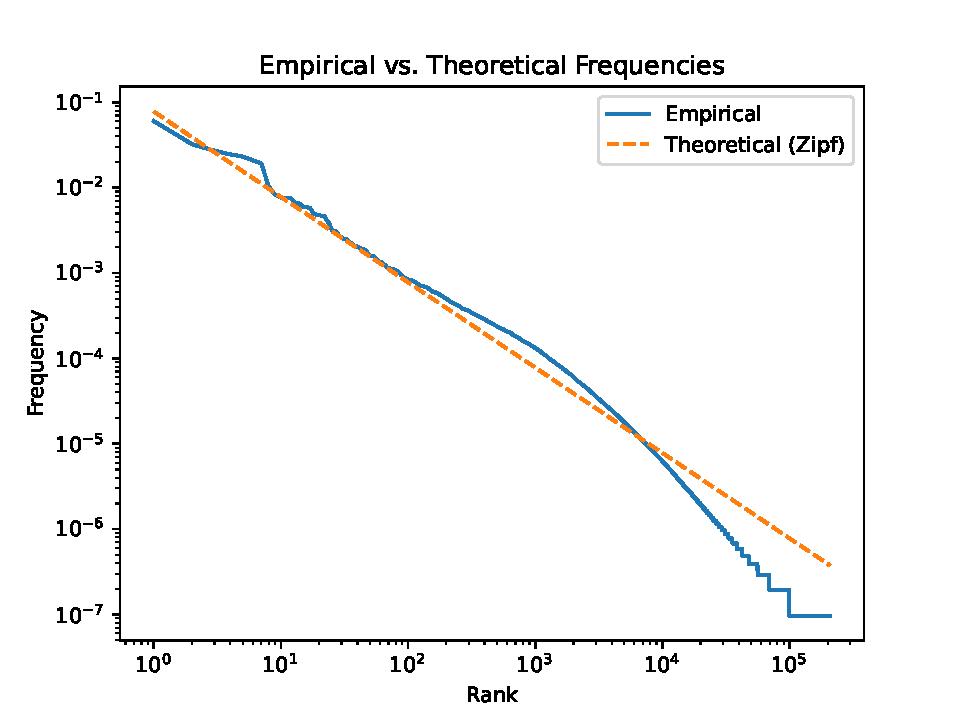
\includegraphics[width=0.45\textwidth]{Task_1_1_fig.pdf}
\caption{Empirical distribution vs. Zipf's law distribution.}
\label{fig:zipf1}
\end{figure}

\begin{figure}[H]
\centering
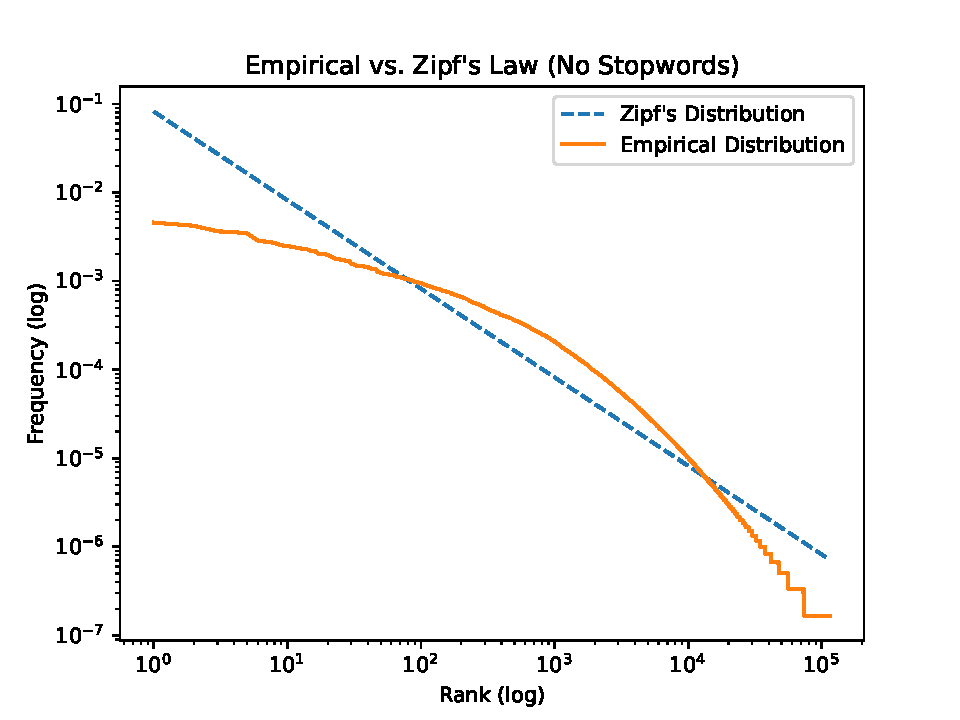
\includegraphics[width=0.45\textwidth]{Task_1_2_fig.pdf}
\caption{Empirical vs. Zipf's law distribution (log-log scale).}
\label{fig:zipf2}
\end{figure}

\begin{figure}[H]
\centering
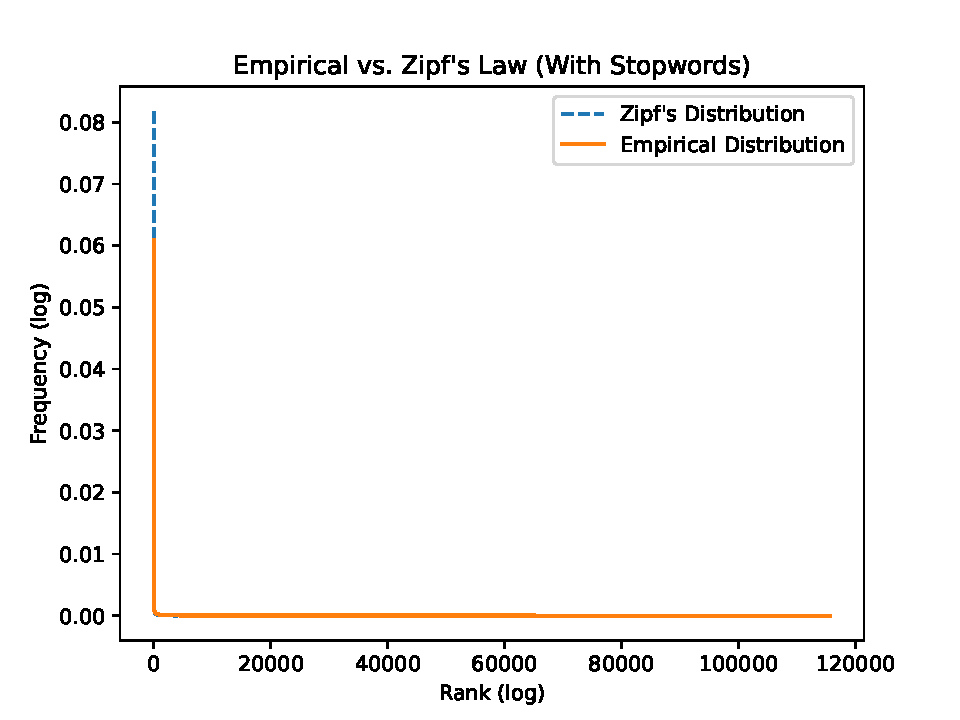
\includegraphics[width=0.45\textwidth]{Task_1_3_fig.pdf}
\caption{Empirical vs. Zipf's law distribution after stop word removal (log-log scale).}
\label{fig:zipf3}
\end{figure}

\section{Task 2 -- Inverted Index}
To construct an inverted index, the passages in \texttt{candidate-passages-top1000.tsv} are processed using the functions developed in Task 1. This involves removing stop words and applying stemming to each token. The output of Task 1 is a two-dimensional list, where each sublist contains tokens from a unique passage. A dictionary is then created in the format \{ \texttt{pid: tokens found in the passage} \}, mapping passage IDs to their tokenized contents.

Next, the inverted index is built by iterating through all tokens and computing their frequency within each passage. The resulting dictionary has the format \{ \texttt{token: \{pid: frequency\}} \}, where each token is a key whose value is another dictionary that maps the passage ID (\texttt{pid}) to its frequency.

This structure allows efficient retrieval of token occurrences, indicating which passages contain a given word and how often.

\section{Task 3 -- Retrieval Models}
This task ranks passages for each query using two models: TF-IDF with cosine similarity and BM25. First, each passage is represented as a TF-IDF vector by combining term frequency (\(\mathrm{tf}(t,p)\)) with inverse document frequency (\(\mathrm{idf}(t)\)). Specifically, we compute
\[
\mathrm{idf}(t) = \log_{10}\!\Bigl(\tfrac{N_{\mathrm{doc}}}{\mathrm{df}(t)}\Bigr).
\]
where \(\mathrm{N_{doc}}\) is the total number of passages and \(\mathrm{df}(t)\) is the number of passages containing \(t\). The cosine similarity between the query’s TF-IDF vector and each candidate passage is then calculated, retaining the top 100 passages. The results are stored in \texttt{tfidf.csv} in the format \texttt{qid,pid,score}.

Next, BM25 is implemented by assigning scores to each query–passage pair with parameters \(k_1 = 1.2\), \(k_2 = 100\), and \(b = 0.75\). Each term’s contribution is derived from its document frequency and its frequency within the passage. The top 100 passages per query are selected and saved in \texttt{bm25.csv} with the same CSV format (without headers).

\section{Task 4 -- Query Likelihood Language Models}
Dirichlet smoothing produces better results than other smoothing techniques because additive smoothing (including Laplace and Lidstone) treats all unseen query tokens equally, potentially overemphasizing their importance. In contrast, Dirichlet smoothing adjusts the smoothing based on background probabilities and document length.

This distinction is illustrated by the query ``what slows down the flow of blood'', tokenized as [\texttt{slow}, \texttt{flow}, \texttt{blood}]. When processed by the three language models, each model ranks passages differently. Below are the top-ranked passages for each model:

\noindent
\textbf{Dirichlet:} ``what slows down the flow of blood \quad What causes esophageal varices? Esophageal varices occur when normal blood flow to your liver is slowed. Liver disease may create scar tissue in the liver which slows the flow of blood. When the blood to your liver is slowed, it begins to back up, leading to an increase of pressure in the major vein (portal vein) that carries blood to your liver.''

\noindent
\textbf{Laplace:} ``what slows down the flow of blood \quad Blood Flow. Blood flow refers to the movement of blood through the vessels from arteries to the capillaries and then into the veins. Pressure is a measure of the force that the blood exerts against the vessel walls as it moves the blood through the vessels. Like all fluids, blood flows from a high pressure area to a region with lower pressure. Blood flows in the same direction as the decreasing pressure gradient: arteries to capillaries to veins...''

\noindent
\textbf{Lidstone:} ``what slows down the flow of blood \quad An aortic aneurysm can also lead to other problems. Blood flow often slows in the bulging section of an aortic aneurysm, causing clots to form. If a blood clot breaks off from an aortic aneurysm in the chest area, it can travel to the brain and cause a stroke...''

Dirichlet smoothing ranks passages that contain all query tokens, whereas Laplace and Lidstone tend to yield a more general discussion of blood flow. Note that Laplace (with \(\epsilon = 1\)) performs worse than Lidstone (with \(\epsilon = 0.1\)) because excessive smoothing in Laplace pushes less relevant passages higher.

Both Laplace and Lidstone smoothing use additive smoothing to ensure that unseen tokens are assigned nonzero probability. They share the generic formula shown in Equation~\ref{eq:additive} (with \(\epsilon=1\) in Laplace):

\begin{equation}
P(W \mid D) = \frac{\mathrm{tf}_{(w,D)} + \epsilon}{|D| + \epsilon \, |V|}
\label{eq:additive}
\end{equation}

For the Lidstone model, \(\epsilon=0.1\) is chosen because the average document is short and the occurrence of key words (excluding stop words) is typically low. Although a smaller \(\epsilon\) (e.g., 0.01) might sometimes be beneficial, it is not guaranteed.

I contend that setting \(\mu = 5000\) for Dirichlet smoothing is not suitable for these text collections. The Dirichlet smoothing formula (Equation~\ref{eq:dirichlet}) shows that for an average text length of about 56.78 words, the term \(\frac{N}{N+\mu}\) becomes very small and \(\frac{\mu}{N+\mu}\) approaches 1. Consequently, the probability becomes predominantly dependent on the background probability \(P(W \mid C)\), which is undesirable. Therefore, \(\mu = 50\) is a more appropriate value.

\begin{equation}
P = \frac{N}{N + \mu}P(W \mid D) + \frac{\mu}{N + \mu}P(W \mid C)
\label{eq:dirichlet}
\end{equation}

\end{document}
